\section{Wick's Theorem, Path Integral for Free Scalar Field Theory}
\subsection{Review}
We computed the path integral with sources (also known as the generating functional) for the SHO, with action:
\begin{equation}
    S = \int dt \frac{1}{2}\dot{q}^2 - \frac{1}{2}\omega^2q^2 = \int \frac{d\omega}{2\pi}\frac{1}{2}(\omega^2 - m^2)q_\omega q_{-\omega}
\end{equation}
which gave the generating functional:
\begin{equation}
    Z[f] = \int \D q e^{iS + \int dt f(t)q(t)} = Z[0]\exp(-\frac{i}{2}\int \frac{d\omega}{2\pi}\frac{1}{\omega^2 - m^2}f_\omega f_{-\omega})
\end{equation}
the logarithm which gives:
\begin{equation}
    \log Z[f] = -\frac{i}{2}\int \frac{d\omega}{2\pi}\frac{1}{\omega^2 - m^2}f_\omega f_{-\omega} = \frac{i}{2}\int dtdt'(-1)\int \frac{d\omega}{2\pi} \frac{e^{-i\omega(t-t')}}{\omega^2 - m^2} f_\omega f_{-\omega} = \frac{i}{2}\int dt'dt'(-1)G(t-t')f_\omega f_{-\omega}
\end{equation}

We can then generate (connected) correlators by taking functional derivatives $\fd{}{f(t)}$ and then setting the source to $f = 0$. For example:
\begin{equation}
    \bra{0}\mathcal{T}\set{\hat{Q}(t_1), \hat{Q}(t_2)}\ket{0} = \left.\frac{1}{i}\fd{}{f(t_1)}\frac{1}{i}\fd{}{f(t_2)}\log Z[f] \right|_{f=0} = -iG(t_1 - t_t) = G_F(t_1 - t_2)
\end{equation}

\subsection{Evaluating the Green's Function}
Now, let's evaluate the fourier transform:
\begin{equation}
    G(t) = -\int \frac{d\omega}{2\pi}\frac{e^{i\omega t}}{\omega^2 - m^2 + i\e}
\end{equation}
We were dropping the $i\e$s previously, but when evaluating this integral, it becomes relevant for locating the poles of the function. So, we re-introduce it here (we know what the correct perscription of the poles for the Feynman correlator is).

The poles are located at $\omega_\pm = \pm \sqrt{m^2 - i\e}$. They are close to $\pm m$, but they are shifted from the real axis. How do we treat these $i\e$? We don't care about the magnitude, only that it is a positive number. We consider a Taylor expansion:
\begin{equation}
    \omega_\pm = \pm m\sqrt{1 - \frac{i\e}{m}} = \pm m(1 - i\e)
\end{equation}
where we have neglected factors of $m, 2$ as we don't care about the magnitude of $\e$, only its sign. Hence, the poles are at:
\begin{equation}
    \omega_\pm = \pm m(1 - i\e)
\end{equation}
which when sketched graphically:
\begin{center}
    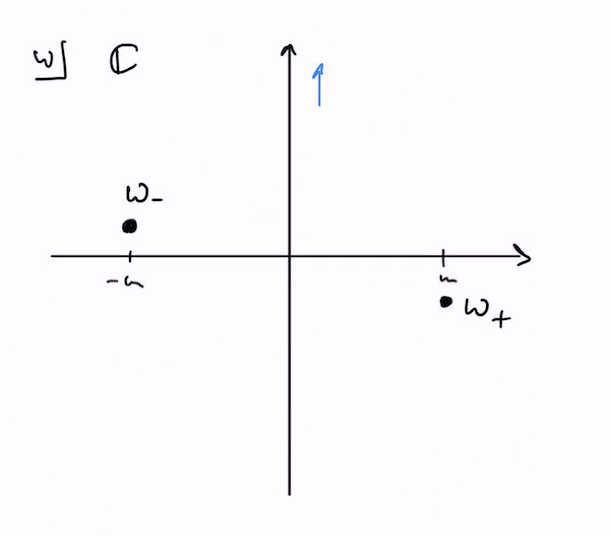
\includegraphics[scale=0.8]{Lectures/Figures/Feynmanpoles.png}
\end{center}

How do we perform this integral? It depends on whether $t$ is positive or negative. If $t < 0$, then we want to close the contour in the lower half plane. Why this choice? We are concretely interested in the integral from $-\infty$ to $\infty$, i.e. $C_1^A$. For this, we like to have a closed contour in the complex plane to carry out the integrals using residue theorems. We use Jordan's lemma. The integral over the semicircular part $C_1^B$ vanishes - as long as $\omega$ has a negative imaginary part, when we push the $C_1^B$ to be a sufficiently large arc to infinity ($e^{i\omega t} = e^{\omega t} = e^{-\abs{t}\omega} \stackrel{\omega\to\infty}{\to} 0$). So, this total closed contour is precisely equal to the integral over the real line.

\begin{center}
    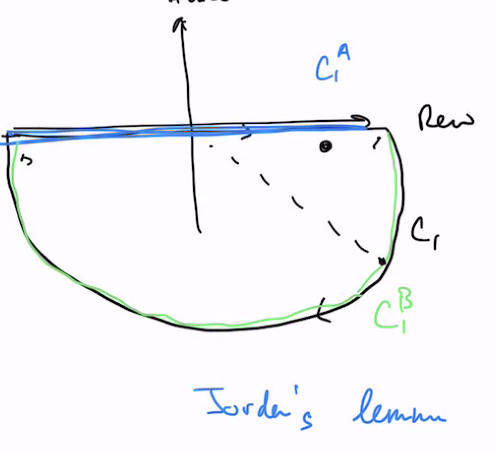
\includegraphics[scale=0.8]{Lectures/Figures/lowerhalfcontour.png}
\end{center}

By the residue theorem:
\begin{equation}
    G(t) = -\int_{C_1}\frac{d\omega}{2\pi}\ldots = 2\pi i \text{Res}(\frac{1}{2\pi}\frac{e^{-i\omega t}}{(\omega - \omega_+)(\omega - \omega_-)}, \omega \to \omega_+) = i\frac{e^{-i\omega_+ t}}{\omega_+ - \omega_-} = i\frac{e^{-im\abs{t}}}{2m}
\end{equation}

If $t > 0$, we close the contour in the upper-half plane:
\begin{center}
    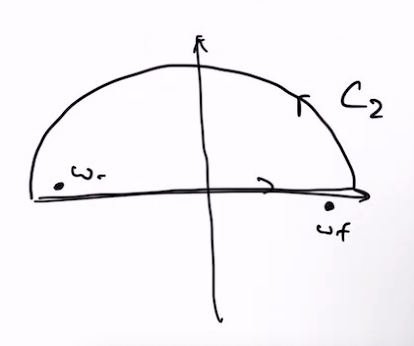
\includegraphics[scale=0.8]{Lectures/Figures/upperhalfcontour.png}
\end{center}
So:
\begin{equation}
    G(t) = -\int_{C_2}\frac{d\omega}{2\pi}\ldots = -2\pi i \text{Res}(\frac{1}{2\pi}\frac{e^{i\omega t}}{(\omega - \omega_+)(\omega - \omega_-)}, \omega \to \omega_-) = -i\frac{e^{i\omega_-t}}{\omega_- - \omega_+} = i\frac{e^{-imt}}{2m} = i\frac{e^{-im\abs{t}}}{2m}
\end{equation}

\subsection{Higher-Point Functions and Wick's Theorem}
What about higher point functions? Let's study the 4-point function. (All odd higher point functions vanish due to symmetry).

\begin{equation}
    \bra{0}\mathcal{T}\{\hat{Q}(t_1)\hat{Q}(t_2)\hat{Q}(t_3)\hat{Q}(t_4)\}\ket{0} = \left.\frac{1}{Z}\frac{1}{(i)^4}\fd{}{f(t_1)}\fd{}{f(t_2)}\fd{}{f(t_3)}\fd{}{f(t_4)} Z[f]\right|_{f=0}
\end{equation}

The connected 4-point function (denoting $\p_i = \fd{\delta}{\delta f(t_i)}$):
\begin{equation}
    \begin{split}
        \p_{1}\p_{2}\p_{3}\p_{4}\log Z &= \p_1\p_2\p_3\left(\frac{\p_4 Z}{Z}\right) 
        \\ &= \p_1\p_2\left(\frac{\p_3\p_4 Z}{Z} - \frac{\p_3 Z}{Z}\frac{\p_4 Z}{Z}\right)
        \\ &= \left.\p_1\left(\frac{\p_2\p_3\p_4 Z}{Z} - \frac{\p_3\p_4 Z}{Z}\frac{\p_2 Z}{Z} - \frac{\p_2\p_3 Z \p_4 Z}{Z^2} - \frac{\p_3 Z\p_2\p_4 Z}{Z^2} + 2\frac{\p_2Z \p_3 Z\p_4 Z}{Z^2}\right)\right|_{f=0}
        \\ &= \frac{\p_1\p_2\p_3\p_4 Z}{Z} - \frac{\p_3\p_4 Z}{Z}\frac{\p_1\p_2 Z}{Z} - \frac{\p_2\p_3 Z \p_1\p_4 Z}{Z^2} - \frac{\p_1 \p_3 Z \p_2 \p_4 Z}{Z^2}
    \end{split}
\end{equation}
An observation; only terms with an even number of derivatives will survive when we set $f = 0$, which we use in the last equality (we discard all terms with an odd number of derivatives). We use this observation in the last equality. Thus:
\begin{equation}
    \begin{split}
        &\bra{0}\mathcal{T}\{\hat{Q}(t_1)\hat{Q}(t_2)\hat{Q}(t_3)\hat{Q}(t_4)\}\ket{0}_C 
        \\ &= \bra{0}\mathcal{T}\{\hat{Q}(t_1)\hat{Q}(t_2)\hat{Q}(t_3)\hat{Q}(t_4)\}\ket{0} - \bra{0}\hat{Q}(t_4)\hat{Q}(t_3)\ket{0}\bra{0}\hat{Q}(t_2)\hat{Q}(t_1)\ket{0} - \ldots
        \\ &= \bra{0}\mathcal{T}\{\hat{Q}(t_1)\hat{Q}(t_2)\hat{Q}(t_3)\hat{Q}(t_4)\}\ket{0} - G_F(t_4-t_3)G_F(t_2-t_1) - G_F(t_4-t_2)G_F(t_3-t_1) - G_F(t_4-t_1)G_F(t_3-t_2)
    \end{split}
\end{equation}
i.e. the connected correlation function is just the 4 point function minus all possible pairs of contractions. Note that this result is true beyond the simple harmonic oscillator (there was no dependence on the actual form of $Z$ here), and is true of any theory where there is a $Q \leftrightarrow -Q$ $\mathbb{Z}_2$ symmetry.

For the SHO (and ``Gaussian'' theories more generally), we found that $\log Z \propto f^2$, i.e. all \emph{connected} higher-point functions vanish. This gives us a way to express the four-point function in terms of the two-point functions:
\begin{equation}
    \bra{0}\mathcal{T}\{\hat{Q}(t_1)\hat{Q}(t_2)\hat{Q}(t_3)\hat{Q}(t_4)\}\ket{0} = G_F(t_4-t_3)G_F(t_2-t_1) + G_F(t_4-t_2)G_F(t_3-t_1) + G_F(t_4-t_1)G_F(t_3-t_2)
\end{equation}
Or, phrased another way; in terms of all contractions. In PS3, we showed this using a very different (brute force) approach. The proof we did here is much easier to generalize to higher-point functions. This is generally known as \emph{Wick's theorem}, which (if the connected correlation functions vanish) we can express higher point functions as all contractions of lower-degree correlation functions.

\subsection{Path Integral for the Free Scalar}
Our action for the free scalar field is:
\begin{equation}
    S = \int dt \frac{1}{2}\dot{q}^2 - \frac{1}{2}m^2q^2 \to S = \int dt d^dx \frac{1}{2}(-\p_\mu \phi)^2 - \frac{1}{2}m^2\phi^2
\end{equation}
Where the distinction from the SHO case is we have changed from the classical coordinate $q(t)$ to the classical field $\phi(t, \v{x})$, or in terms of quantum operators, from the operator $\hat{Q}(t)$ to the field operator $\hat{\phi}(t, \v{x})$. 

We again consider a generating functional and sources, where we promote the source $f(t)$ in the SHO case to the source $J(t, \v{x}) = J(x)$. Thus, we have the action plus source:
\begin{equation}
    S + \int d^{d+1}x J(x)\phi(x).
\end{equation}
The path integral is an integral over all histories $\phi(t, \v{x})$. We see this in the integral $\int \mathcal{D}\phi$ for the generating functional:
\begin{equation}
    Z[J] = \int \D \phi e^{i\int d^{d+1}L + J(x) \phi(x)}
\end{equation}
We can generate correlators like before, e.g.:
\begin{equation}
    \bra{0}\mathcal{T}\set{\hat{\phi}(t_1, \v{x}_1)\hat{\phi}(t_2, \v{x}_2)}\ket{0} = \left.\frac{1}{Z}\frac{1}{i}\fd{}{J(x_1)}\frac{1}{i}\fd{}{J(x_2)}Z[J]\right|_{J=0}.
\end{equation}
The free scalar field will turn out to have a very similar solution to that of the SHO (both are ``Gaussian''):
\begin{equation}
    S + \int d^{d+1}J(x)\phi(x) = \int \frac{d^{d+1}p}{(2\pi)^{d+1}}\left(-\frac{1}{2}\right)(p^2 + m^2)\phi_p\phi_{-p} + \frac{1}{2}(J_p\phi_{-p} + \phi_pJ_{-p})
\end{equation}
Where $p^2 = -(p_0)^2 + \v{p}^2 = -\omega^2 + \v{p}^2$ and $\phi_p = \int d^{d+1}x e^{-ip_\mu x^\mu}\phi(x)$ and similarly for $J_p$. Like we did for the SHO, we complete the square:
\begin{equation}
    \begin{split}
        S[\phi] + \int d^{d+1}J(x)\phi(x) = \int \frac{d^{d+1}p}{(2\pi)^{d+1}} \left(-\frac{1}{2}\right)(p^2+ m^2)\left(\phi_p - \frac{1}{p^2 + m^2}J_p\right)\left(\phi_{-p} - \frac{1}{p^2 + m^2}J_{-p}\right) + \frac{1}{2}J_p\frac{1}{p^2 + m^2}J_{-p}
        \\ &= S[\bar{\phi}] + \int \frac{d^{d+1}p}{(2\pi)^{d+1}}\frac{1}{2}J_p\frac{1}{p^2 + m^2}J_{-p}
    \end{split}
\end{equation}
To compute $Z$, we perform the change of variable $\phi_p \to \bar{\phi}_p = \phi_p - \frac{1}{p^2 + m^2}J_p$, so:
\begin{equation}
    Z[J] = \int \D\bar{\phi}e^{iS[\bar{\phi}]}e^{i\int \frac{d^{d+1}p}{(2\pi)^{d+1}}\frac{1}{2}J_p\frac{1}{p^2 + m^2}J_{-p}} = Z[0]\exp(\frac{i}{2}\int \frac{d^{d+1}p}{(2\pi)^{d+1}}J_p\frac{1}{p^2 + m^2}J_{-p})
\end{equation}
So we've basically solved the free scalar QFT, in the sense that we have a generating functional for it. As with the QHO, we observe that $\log Z[J]$ is very simple:
\begin{equation}
    \log Z[J] = \log Z[0] + \frac{i}{2}\int \frac{d^{d+1}p}{(2\pi)^{d+1}}J_p\frac{1}{p^2 + m^2}J_{-p} = \log Z[0] + frac{i}{2}\int \frac{d^{d+1}p}{(2\pi)^{d+1}}J_pG_F(p)J_{-p}
\end{equation}
i.e. since $\log Z[J] \sim J^2$, so we have that higher connected correlation functions ($n > 2$) vanish and Wick's theorem applies! Thus higher point functions can be written as contractions, which will just be functions of the two-point functions (all higher-point functions are determined by the two-point functions). I.e.:
\begin{equation}
    \bra{0}\mathcal{T}\{\hat{\phi}_1, \hat{\phi}_2, \hat{\phi}_3, \hat{\phi}_4\}\ket{0} = \avg{12}\avg{34} + \avg{13}\avg{24} + \avg{14}\avg{23}
\end{equation}

In position space:
\begin{equation}
    \log Z[J] = \frac{i}{2}\int d^{d+1}xd^{d+1}x'\left(\int \frac{d^{d+1}p}{(2\pi)^{d+1}}\frac{e^{-ip(x-x')}}{p^2 + m^2 - i\e}\right) J(x)J(x') = \frac{i}{2}\int d^{d+1}xd^{d+1}x' G_F(x-x')J(x)J(x')
\end{equation}
so we recover the same result we found in the Hamiltonian approach using the path integral approach. To expand slightly on the last point, the Feynman's Green function is the time-ordered correlation function:
\begin{equation}
    G_F(x -x') = \bra{0}\mathcal{T}\{\hat{\phi}(x), \hat{\phi}(x')\}\ket{0} = \left.\frac{1}{Z}\frac{1}{i}\fd{}{J(x)}\frac{1}{i}\fd{}{J(x')} \log Z\right|_{J=0} = -i\int \frac{d^{d+1}p}{(2\pi)^{d+1}}\frac{e^{-ip(x-x')}}{p^2 + m^2 - i\e}
\end{equation}
where in the second-to-last equality we note that for two-point functions, connected correlation functions are the unconnected correlation functions because the one-point functions vanish.

\subsection{Looking Ahead}
This is a great starting point; we have a fully solved (free) QFT. But, the world would be pretty uninteresting if it was free. We will start to look at interactions, which are generally unsolvable. But for sufficiently weak interaction, a lot of our machinery will come in useful.

As a teaser, we can consider a $\phi^3$ term:
\begin{equation}
    S = S_{\text{free}} + \lambda\int \phi^3
\end{equation}
which breaks the $\mathbb{Z}_2$ symmetry, so we see that three-point functions will now be nonzero:
\begin{equation}
    \bra{0}\hat{\phi}_1\hat{\phi}_2\hat{\phi}_3 \sim \lambda \neq 0.
\end{equation}
How do we attack this? We will consider:
\begin{equation}
    \int \D \phi e^{iS_{\text{free}}}e^{iS_{text{int}}}
\end{equation}
with $e^{iS_{text{int}}} \approx 1+ i\lambda \int \phi^3$ and roughly this corresponds to taking expectations of the interactions with the free theory:
\begin{equation}
    \bra{0}\hat{\phi}_1\hat{\phi}_2\hat{\phi}_3 \approx \bra{0}\phi\phi\phi \left(i\lambda \int \phi^3 \right)\ket{0} \neq 0 
\end{equation}